% ************************************************************************
%
% Bookmark
%
% ************************************************************************
\documentclass[10pt]{report}
\usepackage[dutch]{babel}
\usepackage{pagecolor}
\usepackage{graphicx}

\topmargin         -30.0mm
\leftmargin        0.0mm
\pdfpagewidth     60.0mm
\paperwidth     60.0mm
\pdfpageheight   240.0mm
\paperheight    240.0mm
\textheight      220.0mm
\textwidth        50.0mm
\hoffset         -43.0mm

% ************************************************************************
\definecolor{backgroundColor}{RGB}{255, 255, 232}
\begin{document}
	\newpagecolor{backgroundColor}
\selectlanguage{dutch}
\pagestyle{empty}
\setlength{\leftmargini}{0em}
% ************************************************************************

\begin{center}
	
  	{\Large\bf Uitnodiging}

  	\bigskip

  	voor het bijwonen van de openbare verdediging van het proefschrift

  	\bigskip
  	\bigskip
	
  	{\Large\bf  Methods for Automated Neuron Image Analysis}% Methoden voor geautomatiseerde beeldanalyse van neuronen

  	\bigskip
  	\bigskip
  
  	Dinsdag 29 januari 2019\\om 13:30 uur
  
  	\bigskip
  	\bigskip
  
  	Professor Andries Querido zaal\\
  	Onderwijscentrum\\%[0.5em]
  	Erasmus MC Rotterdam
  
  	\bigskip
  	\bigskip
  
 	Receptie na afloop van de plechtigheid
  
 	\bigskip
 	\bigskip

	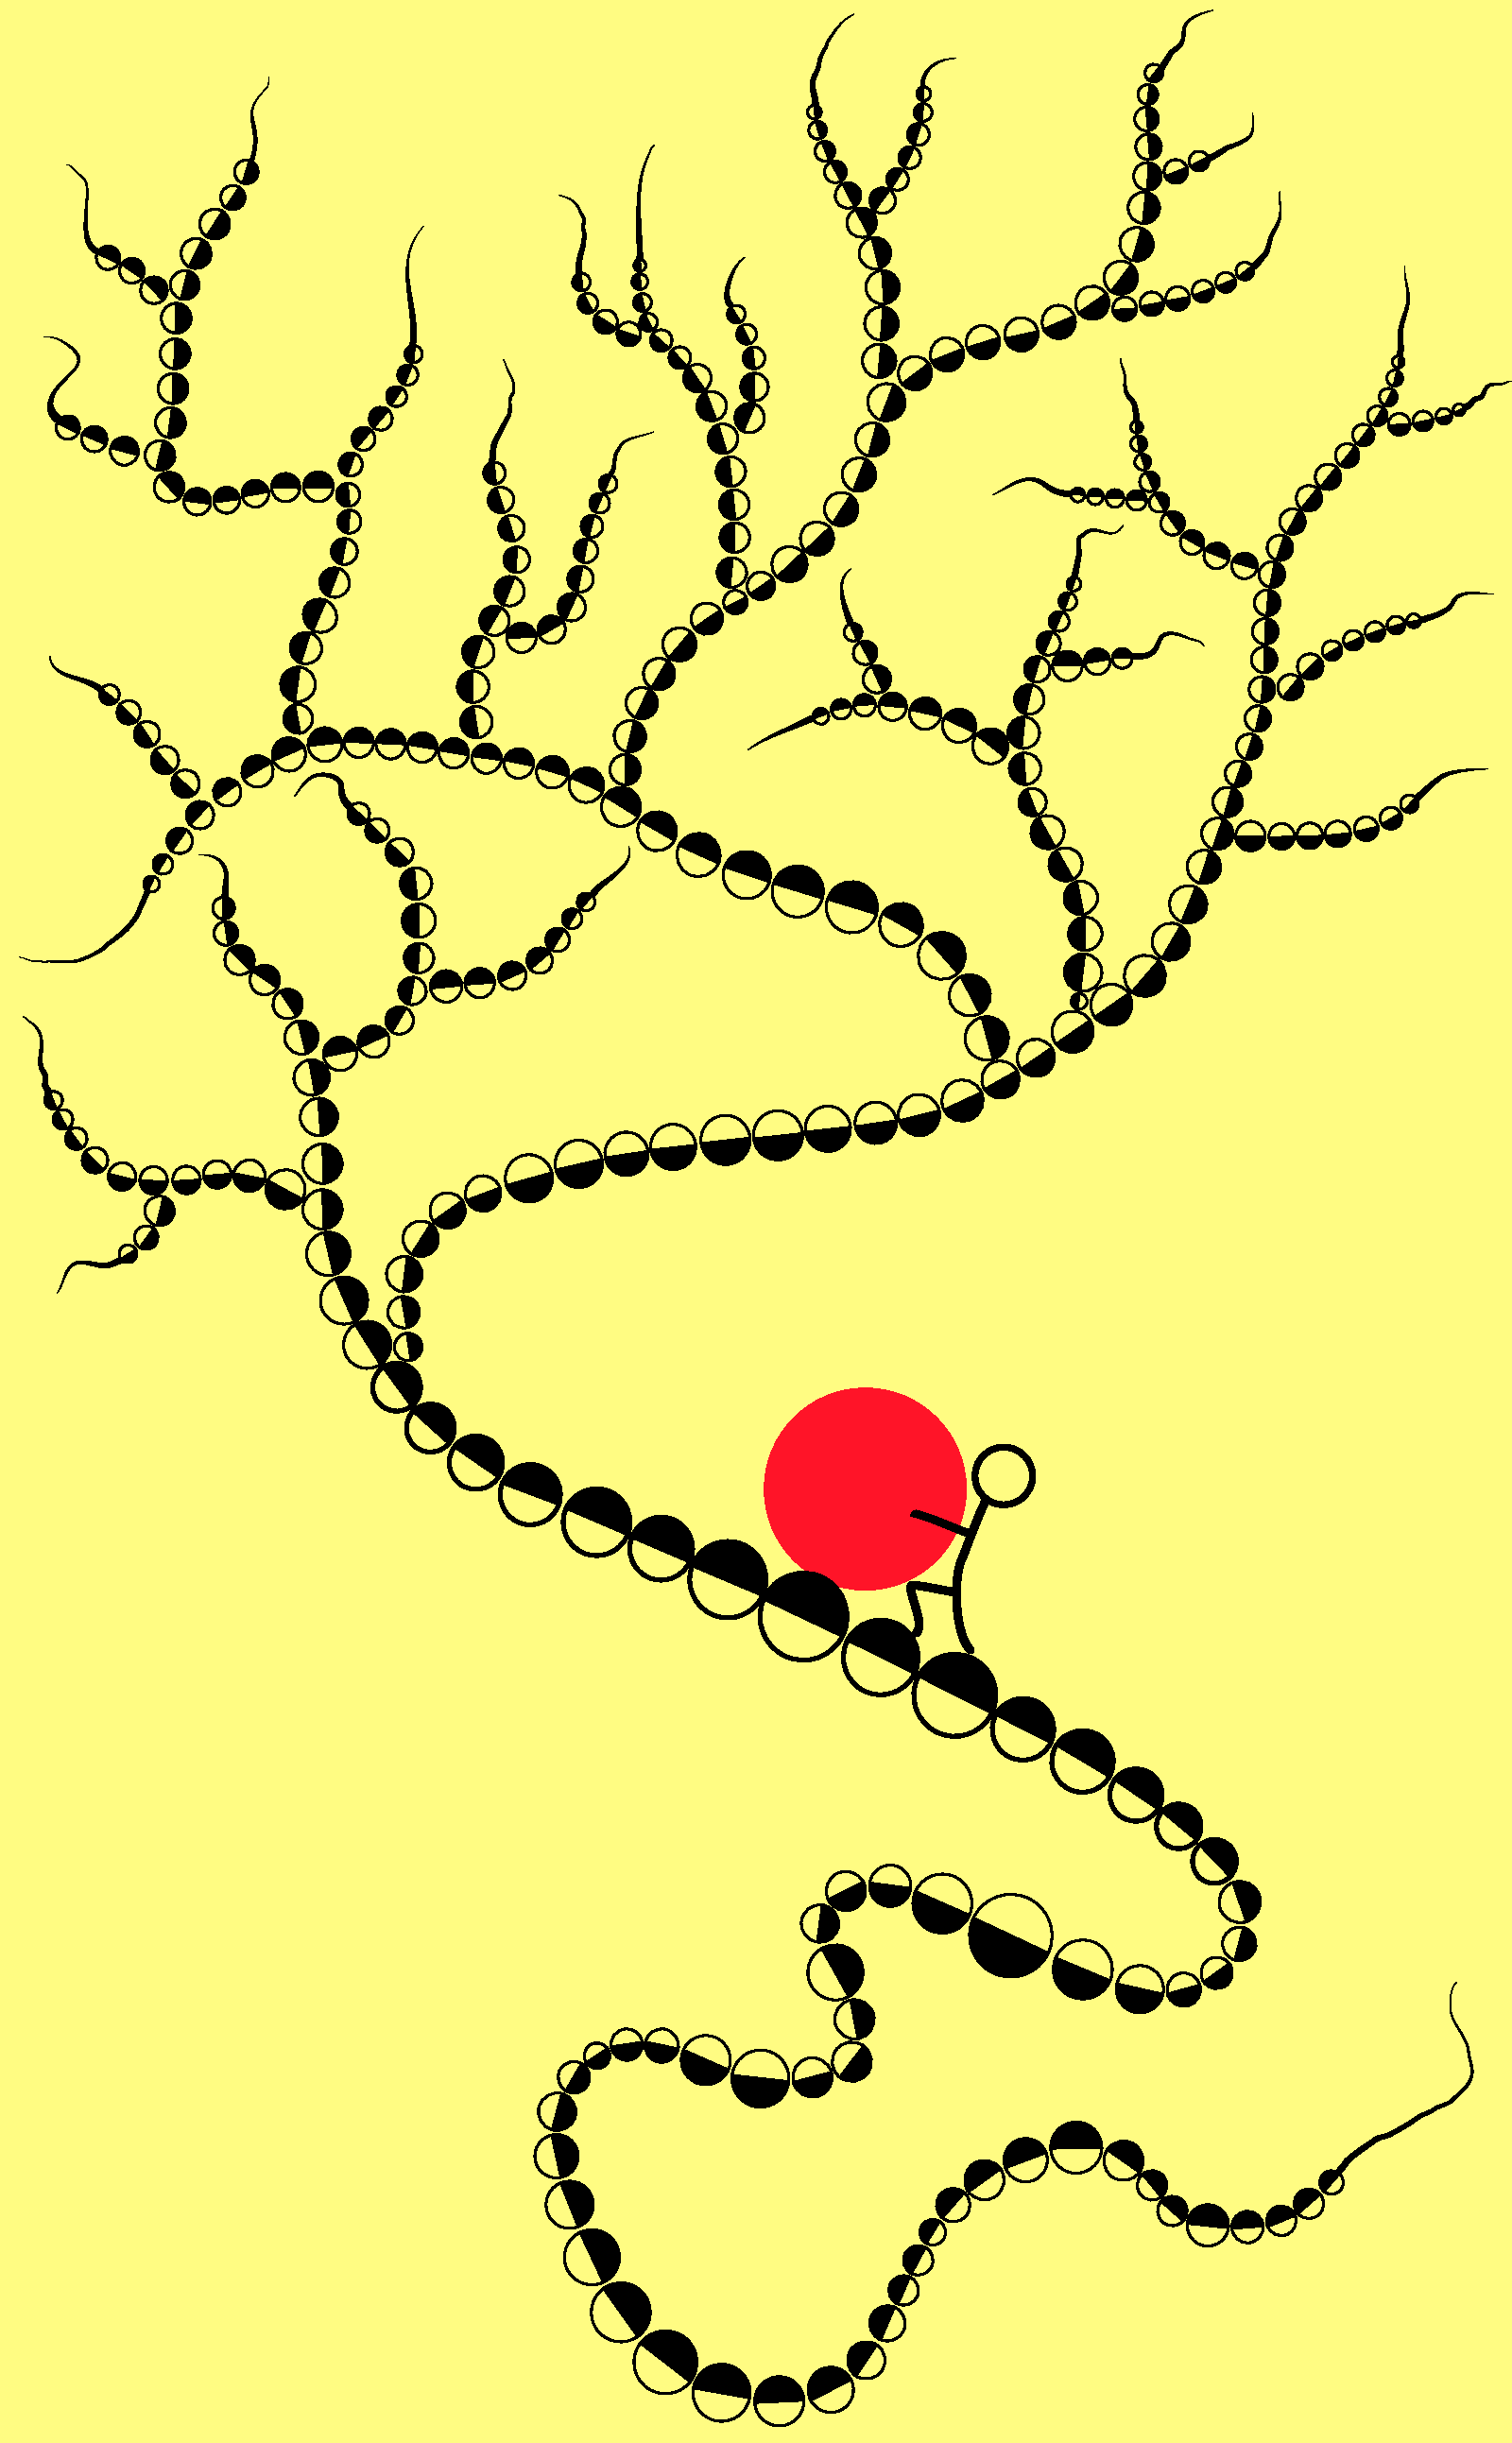
\includegraphics[width=0.85\textwidth]{syziphus}

	\bigskip
	\bigskip

  	{\Large Miroslav Radojevi\'{c}}\\[0.5em]
  	Rabenhauptstraat 24\\
  	9725CD Groningen\\
  	miroslav.radojevic@gmail.com\\[1em]
  	{\normalsize Paranimfen:}\\[0.5em]
  	An\dj elka Ze\v{c}evi\'{c}\\
  	andjelkaz@matf.bg.ac.rs\\[0.5em]
  	Eugene Katrukha
  	y.katrukha@uu.nl
  
\end{center}

% ************************************************************************
\end{document}
% ************************************************************************
